\documentclass[border=4pt]{standalone}
% Shared typography and colours for the standalone figures.
\usepackage{unicode-math}
\setmainfont{TeX Gyre Termes}
\setmathfont{TeX Gyre Termes Math}
\usepackage{tikz}
\usetikzlibrary{arrows.meta,positioning,calc,decorations.pathreplacing}
\usepackage{pgfplots}
\pgfplotsset{compat=1.18}

% One colour per element or subsystem. Record the mapping in
% the working repository conventions and use it identically in every figure.
\definecolor{elemA}{HTML}{1F5FA8}
\definecolor{elemB}{HTML}{B8461B}
\definecolor{elemC}{HTML}{2E7D32}
\definecolor{elemD}{HTML}{6A4C93}
\definecolor{frameline}{HTML}{555555}

\begin{document}
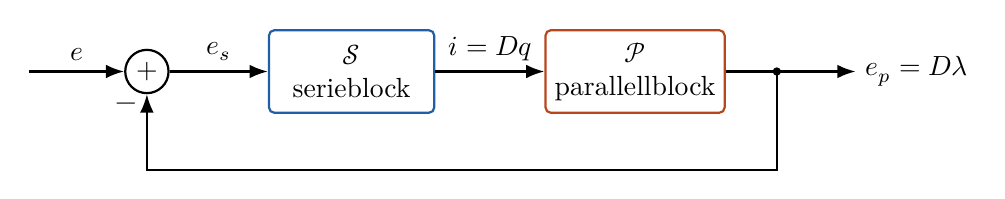
\begin{tikzpicture}[>=Latex,thick,
  block/.style={draw,rounded corners=2pt,minimum width=2.1cm,minimum height=1.05cm,align=center}]
  \node[draw,circle,minimum size=0.55cm,inner sep=0pt] (sum) at (0,0) {$+$};
  \node[block,draw=elemA] (series) at (2.6,0) {$\mathcal S$\\serieblock};
  \node[block,draw=elemB] (parallel) at (6.2,0) {$\mathcal P$\\parallellblock};
  \draw[->] (-1.5,0) -- node[above] {$e$} (sum);
  \draw[->] (sum) -- node[above] {$e_s$} (series);
  \draw[->] (series) -- node[above] {$i=Dq$} (parallel);
  \draw[->] (parallel) -- (9,0) node[right] {$e_p=D\lambda$};
  \fill (8,0) circle (1.5pt);
  \draw[->] (8,0) -- (8,-1.25) -- (0,-1.25) -- node[left,pos=0.83] {$-$} (sum);
\end{tikzpicture}
\end{document}
